
\begin{SCfigure}[1][htb]
    \centering
    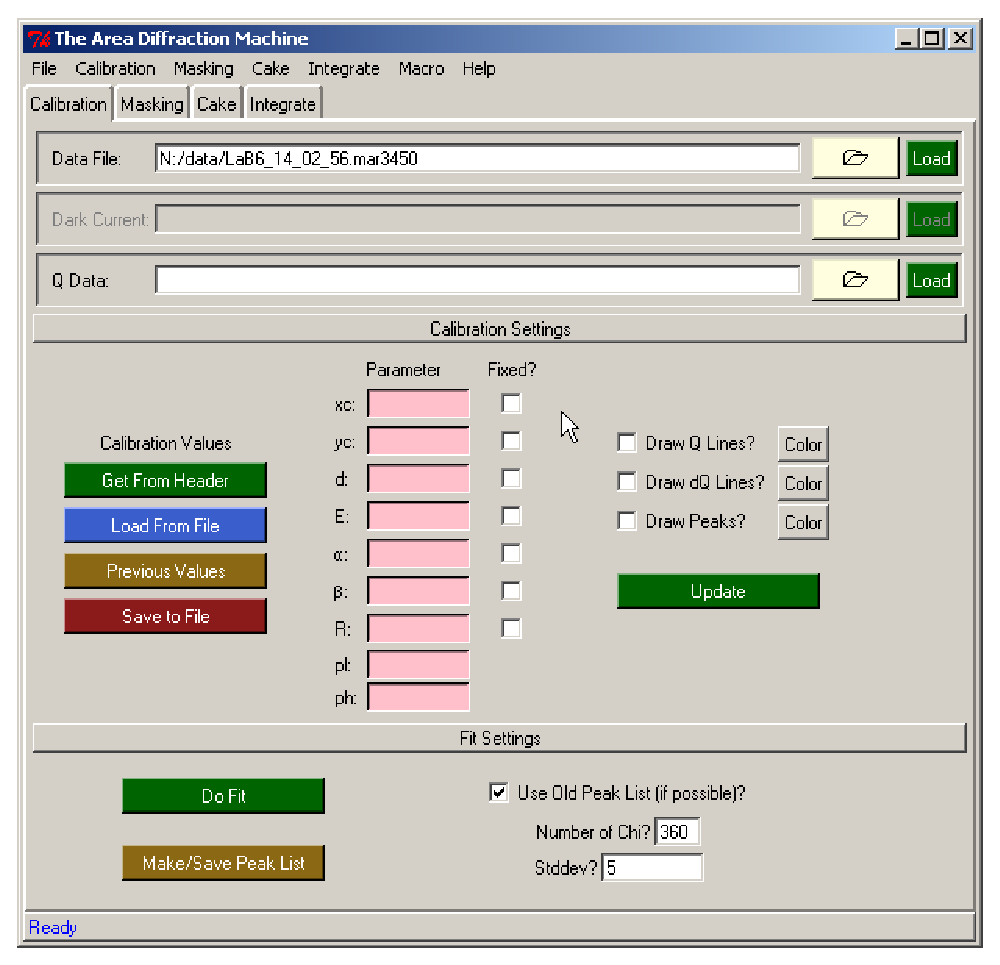
\includegraphics[scale=.75]{figures/calibration_page.eps}
    \caption{A screen shot of the calibration tab to the program.
    This is what you see when you first open up the program. 
    This page allows you to, among other things, load diffraction
    data into the program.`} 
    \label{calibration_page}
\end{SCfigure}

When you first open the Area Diffraction Machine up, you
will be presented with the window shown in 
figure~\ref{calibration_page}. The first thing that you
will probably want to do is load some diffraction data into
the program. To do so, you can see the Data File: input.
You can either type in the filename by hand and push the
load button or click on the folder icon to the side and
use the file selector to pick the file that you want.
Once the file is loaded, you will be presented with
the window shown in figure~\ref{diffraction_data_window}

\begin{SCfigure}[1][htb]
    \centering
    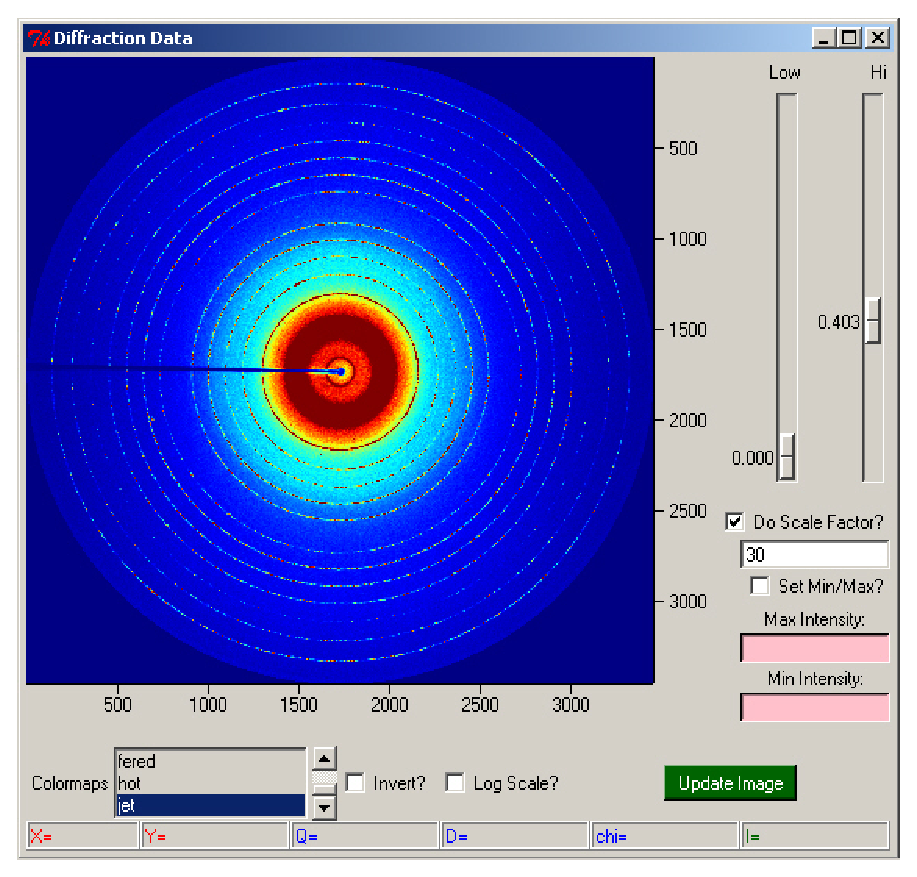
\includegraphics[scale=.75]{figures/diffraction_data_window.eps}
    \caption{A screen shot of the diffraction data window for
    the program. This window will be opened up after a file is 
    loaded. This windows allows you to interact with diffraction 
    data.} 
    \label{diffraction_data_window}
\end{SCfigure}


Once the diffraction data window has opened up, you can use
the window to interact with your diffraction data. With
the window you can
\begin{itemize}
    \item {\em Zoom into the data} - To zoom, left click on
    the data and hold down on the mouse. When you drag the cursor, 
    the program will create a resizing square. When you let go of the
    mouse, the selected square will be used as the outer bound and
    the image will be zoomed into it.
    \item {\em Zoom out of the data} - To unzoom, right click on
    the data.
    \item {\em Pan across the data} - To pan, hold down on shift, than
    right (or left) click on the data and hold down on the mouse. When 
    you move the mouse, the program will pan the image to follow the 
    cursor. When you let go of the mouse, the program will stop panning.
    \item {\em Resize the window} - This will make the diffraction
    image either larger or smaller. To do so, click on the bottom 
    right corner and drag.
    \item {\em Read coordinates for a selected point}
    \item {\em Change the Color Map}
    \item {\em Invert the Color Map}
    \item {\em Log Scale the Color Map}
\end{itemize}


\subsection{File Formats}

The program can load in Mar data: \macroline{.mar3450}, 
\macroline{.mar2300}, and \macroline{.mccd} marccd format.
It can load in standard \macroline{.tiff} data. 
It can load in the ESRF Data Format 
\macroline{.edf}.


\subsection{Loading Multiple Images}


\begin{itemize}
\item Color Map, 
\item Invert
\item Lower than value 
\item Upper than value
\item resize
\end{itemize}
